% Totoro sitting in the snow
% By Noa Hoffmann and Pascal Günthner, 21.12.2020
\documentclass[tikz,11pt]{{standalone}}
\usepackage{calligra}
\usepackage[T1]{fontenc}
\usetikzlibrary{positioning, chains, calc, fit, arrows.meta, shapes}
\usepackage{bigints}

\begin{document}    
        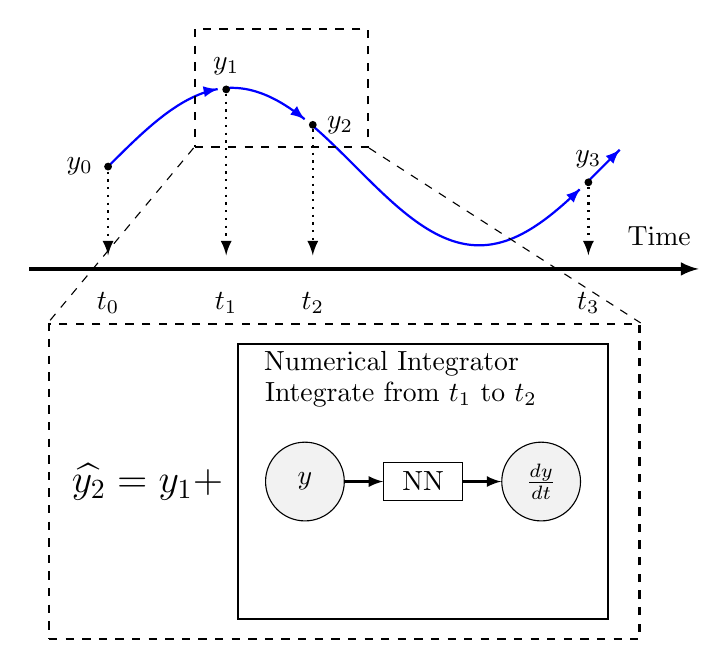
\begin{tikzpicture}[
        item/.style={circle,draw,thick},
        itemc/.style={item,on chain,join},             
        cell/.style={% For the main box
            rectangle, 
            rounded corners=2mm, 
            draw,
            very thick,
            fill=green!10,
            },
        operator/.style={%For operators like +  and  x
            circle,
            draw,
            inner sep=-0.5pt,
            minimum height =.35cm,
            },
        function/.style={%For functions
            ellipse,
            draw,
            inner sep=1pt
            },
        ct/.style={% For external inputs and outputs
            circle,
            draw,
            minimum height =1.cm,
            },
        gt/.style={% For internal inputs
            rectangle,
            draw
            },
        mylabel/.style={% something new that I have learned
            font=\scriptsize\sffamily
            },
        ArrowC1/.style={% Arrows with rounded corners
            rounded corners=.25cm,
            thick,
            },
        ArrowC2/.style={% Arrows with big rounded corners
            rounded corners=.5cm,
            thick,
            },
            ]
         \draw[-latex,thick,draw=blue,domain=0.0:1.4,samples=300,variable=\x] node[circle,fill,inner sep=1pt,label=left:$y_0$](a1){} plot (\x,{sin(deg{\x})});
         \draw[-latex,thick,draw=blue,domain=1.5:2.5,samples=300,variable=\x] plot (\x,{sin(deg{\x})});
         \draw[-latex,thick,draw=blue,domain=2.6:6.0,samples=300,variable=\x] plot (\x,{sin(deg{\x})});
         \draw[-latex,thick,draw=blue,domain=6.1:6.5,samples=300,variable=\x] plot (\x,{sin(deg{\x})});
         \node[circle,fill,inner sep=1pt,label=above:$y_1$](a2) at (1.5,0.98){};
         \node[circle,fill,inner sep=1pt,label=right:$y_2$](a3) at (2.6,0.53){};
         \node[circle,fill,inner sep=1pt,label=above:$y_3$](a4) at (6.1,-0.2){};
         \node[circle,label=below:$t_0$](t0) at (0.,-1.3){};
         \node[circle,label=below:$t_1$](t1) at (1.5,-1.3){};
         \node[circle,label=below:$t_2$](t2) at (2.6,-1.3){};
         \node[circle,label=below:$t_3$](t3) at (6.1,-1.3){};
         \node[circle,label=above:Time](t) at (7,-1.3){};
	  \draw [-latex, very thick] (-1, -1.3) -- (7.5, -1.3);
	  \draw [-latex, thick, dotted] (a1) -- (t0);
	  \draw [-latex, thick, dotted] (a2) -- (t1);
	  \draw [-latex, thick, dotted] (a3) -- (t2);
	  \draw [-latex, thick, dotted] (a4) -- (t3);
         \node [dashed] (rect1) at (2.2, 1) [draw,thick,minimum width=2.2cm,minimum height=1.5cm] {};
	  \begin{scope}[yshift=-4.0cm]
                 \node [dashed] (rect2) at (3.,0) [draw,thick,minimum width=7.5cm,minimum height=4cm] {};
                 \node [] (rect3) at (4.,0) [draw,thick,minimum width=4.7cm,minimum height=3.5cm] {};
	        \node () at (0.5, 0.) {\Large $\widehat{y_2} = y_1 +$};
	        \node () at (3.6, 1.5) {Numerical Integrator};
	        \node () at (3.72, 1.1) {Integrate from $t_1$ to $t_2$};
	            % Draw inputs named ibox#
                    \node[ct, fill=gray!10] (o1) at (5.5,0.0) {$\frac{dy}{dt}$};
	            \node [gt, minimum width=1cm] (ibox3) at (4.,-0.0) {NN};
                    \node[ct, fill=gray!10] (i1) at (2.5,0.0) {$y$};
	  \end{scope}
            \draw [dashed] (rect1.south west) -- (rect2.north west);
            \draw [dashed] (rect1.south east) -- (rect2.north east);
            \draw[thick,-latex] (i1) to (ibox3);
            \draw[thick,-latex] (ibox3) to (o1);
        \end{tikzpicture}
\end{document}
